\documentclass[review]{elsarticle}
% \usepackage[utf8]{inputenc}
% \usepackage{subcaption}
% \usepackage{amsmath}
% \usepackage{listings}
% \usepackage{courier}
% \usepackage{tikz}
% \usepackage{graphicx}
% \usepackage{picins}
% \usepackage{epstopdf}
% 
% 
% \usepackage{lipsum}                        % testo fittizio
% 
% \usepackage[nomarkers]{endfloat}
% 
% \newcommand{\listoflstlistings}{\lstlistoflistings}
% \DeclareDelayedFloat{lstlisting}[flol]{\textbf{List of Listings}}
% 
% \lstset{tabsize=2,language=C++,basicstyle=\footnotesize\tt,keywordstyle=\color{blue}\bfseries}

\journal{Powder Technology}

%%%%%%%%%%%%%%%%%%%%%%%%%%%%%%%%%%%%%%%%%%%%%%%%%%%%%%%%%%%%%%%%%%%%%%%%%%%%%%%%%%%%%%%%%%%%%%%%%%%%%%%%%%%%%%%%%%%%%%%%%%
\begin{document}

%%%%%%%%%%%%%%%%%%%%%%%%%%%%%%%%%%%%%%%%%%%%%%%%%%%%%%%%%%%%%%%%%%%%%%%%%%%%%%%%%%%%%%%%%%%%%%%%%%%%%%%%%%%%%%%%%%%%%%%%%%
\begin{frontmatter}

\title{Identification of DEM Simulation Parameters by Artificial Neural Networks
and Bulk Experiments}

\author[jku]{L.~Benvenuti\corref{cor1}}
\ead{Tel. +43 73224686483}
\ead{luca.benvenuti@jku.at}

\author[dcs]{C.~Kloss}
\ead{christoph.kloss@dcs-computing.com}

\author[jku]{S.~Pirker}
\ead{stefan.pirker@jku.at}

\cortext[cor1]{Corresponding author}

\address[jku]{Johannes Kepler University Linz, Department on Particulate Flow
Modelling, Altenbergerstrasse 69, 4040, Linz, Austria}

\address[dcs]{DCS Computing GmbH, Altenbergerstr. 66a - Science Park, 4040 Linz,
Austria}

%%%%%%%%%%%%%%%%%%%%%%%%%%%%%%%%%%%%%%%%%%%%%%%%%%%%%%%%%%%%%%%%%%%%%%%%%%%%%%%%%%%%%%%%%%%%%%%%%%%%%%%%%%%%%%%%%%%%%%%%%%
\begin{abstract}
In Discrete Element Method ($DEM$) simulations, particle-particle contact laws
determine the macroscopic simulation results. Particle based contact laws, in
turn, commonly rely on semi-empirical parameters, which can be hardly obtained
by direct microscopic measurements.
In this study we present a methodology for the identification of
$DEM$ simulation parameters by linking the macroscopic experimental results to the
microscopic numerical parameters by artificial neural networks.
In a first step, a series
of $DEM$ simulations with varying simulation parameters are used to train a feed
forward artificial neural network by backward propagation reinforcement. In a
second step, this artificial neural network is utilized to predict the
macroscopic ensemble behaviour in dependence of additional sets of particle
based simulation parameters.
As a result, a comprehensive database is obtained,
which links particle based simulation parameters to a specific macroscopic
bulk behaviour of the ensemble.
The trained artificial neural network is able to predict the behaviour of
additional sets of input parameters accurately and highly efficient.
Furthermore, this methodology can be applied to
identify $DEM$ material parameters in a generic way.
For each set of calibration experiments, the training of the neural network has
to be performed just once. 
After the training, the neural network provides a generic link between the macroscopic 
experimental results and the microscopic $DEM$ simulation parameters.
By the help of these experiments, the $DEM$ simulation parameters of a specific
non-cohesive granular material can be identified.

\end{abstract}

\begin{keyword}
Discrete Element Method ($DEM$) Simulations \sep Parameter Identification \sep Artificial Neural Networks
\end{keyword}
\end{frontmatter}
%%%%%%%%%%%%%%%%%%%%%%%%%%%%%%%%%%%%%%%%%%%%%%%%%%%%%%%%%%%%%%%%%%%%%%%%%%%%%%%%%%%%%%%%%%%%%%%%%%%%%%%%%%%%%%%%%%%%%%%%%%

%************************************************
\section{Highlights}
\label{sec:highlights}
%************************************************
\begin{itemize}
  \item{We trained an Artificial Neural Network by DEM simulations with varying
  parameters}
  \item{The Artificial Neural Network then predicts granular bulk behaviour}
  \item{By comparison with bulk experiments DEM simulation parameters are
  identified}
  \item{This DEM parameter identification can be applied to different bulk
  behaviours}
  \item{This DEM parameter identification can be applied to different granular
  materials}
\end{itemize}
%************************************************

%%************************************************
\section{Introduction}
\label{sec:introduction}
%************************************************


Discrete Element Method ($DEM$) simulations are widely used to picture particle
behaviour in these granular processes.
$LIGGGHTS$ is one of the most powerful open source $DEM$ simulation software packages available. 
The models it can analyze are described in detail in the literature, see Kloss
et al. \cite{RefWorks:136}, while a useful example is provided by the shear cell tester 
simulation developed by Aigner et al. \cite{RefWorks:139}.
This approach try to solve the issue of particle-particle interaction. 
From the experimental point of view, we are focusing
on the bulk behaviour of the materials analysed.
From that we investigated the relationship with the particle-particle $DEM$
contact parameters.
We tried to obtain simulations ideally perform, with the correct parameters, 
the same macroscopic behaviour of the experiments, the static angle of repose
($AOR$) and Schulze ring shear cell tester ($SRSCT$). That allowed us to later
compare numerical and experimental results, as suggested by Ai et al.
\cite{RefWorks:131}.
We could identify the most suitable value for each $DEM$ parameter 
investigated performing huge numbers of simulations. Each will have a different
value. Regrettably, many parameters contribute to define the numerical bulk behaviour. Performing and investigate the 
more than $10^8$ simulations required was out of the scope of this paper.
Instead, as suggested by Vaferi et al. \cite{RefWorks:150}, we harnessed Artificial Neural Networks ($NN$) for their
stability and reliability with non-linear systems like ours.
Furthermore, the main aim of this work was to improve the characterization 
of several $DEM$ parameters for non-spherical particles. 
From the performed simulations bulk representative parameters were extracted. 
They provide the information for the output layer of the $NN$. Instead the $DEM$ 
parameters of the same simulations provided the information for the input layer. 
Once trained, these $NN$ were fed with random combinations of $DEM$ parameters,
and they provided numerical bulk representative parameters for each
of these combinations.
Those were compared with the experimental results. A portion of the combinations
(ca. 0.1\%) had parameters matching with the experiments.
We kept these combinations as working solutions.

%\section{Modelling Pre-requisites}
\label{sec:modellingprerequisites}

\subsection{Macroscopic Experiments}
\label{subsec:Macroscopicexperiments}

The first step of the procedure was using a SRSCT (see Schulze
\cite{RefWorks:142}) to characterize particle flow properties, especially the complete yield locus.
We obtained for each of the twelve load conditions three values representative of the bulk behaviour: bulk density ($\rho_b$),
coefficient of internal friction in the pre-shear phase $ (\mu_{psh})$ and
coefficient of internal friction in the shear phase  $ (\mu_{sh})$.
Furthermore, to recreate the repose angle observed in a pile of the real material, 
we performed angle of repose ($AOR$) tests, as the $AOR$ was the fourth
behaviour value.
Moreover, we sieved the materials samples to obtain the size distribution of the
particles. Six different sifters have been used.

\subsection{Discrete element method}
\label{subsec:dem}
For the sinter fine used in this work 
Di Renzo and Di Maio \cite{RefWorks:145} suggested using the non-linear Hertzian model without cohesion for 
the particle-particle and particle-wall contacts. 
In this granular model the shear force is a "history" effect that accounts for the tangential displacement 
("tangential overlap") between the particles for the duration of contact. 
The tangential force component is truncated to fulfil $F_{t,ij} \leq \mu_s
F_{n,ij}$,
where $\mu_s$ is the coefficient of sliding friction, one of the particle based
$DEM$ parameter we investigated. 
An ulterior parameter was the coefficient of rolling friction ($\mu_r$). 
For coarse not round particles is a critical parameter and describes inter-particle 
friction in medium to dense granular flows simulations. It is proportional to the 
torque counteracting the rotation of the particle. The $\mu_r$ parameter enters the 
equations according to the elasto-rolling resistance model presented by Wensrich and 
Katterfeld \cite{RefWorks:87}. 
The maximum magnitude of rolling resistance torque is $T_{r~max} = \mu_r R_r
|\tilde{F_n}|$, where $R_r$ is the equivalent radius and $F_n$ the normal force.
The last two particle based $DEM$ parameter we investigated were the particle density 
($\rho_p$) and the coefficient of restitution ($COR$).

\subsection{Artificial Neural Networks}
\label{subsec:ann}

In this paper, we first use Neural Networks ($NN$) to fit the $DEM$ numerical
simulation data, and then to process vast amount of parameters combinations. 
They map combinations of input data into convenient outputs (fitting). 
There is a variety of types of $NN$, remarkably the Feedforward ($FF$) . 
To recognize not linearly separable data the standard linear perceptron $NN$ 
has been modified into \textit{FF Multilayer Perceptron Neural Networks (MLPNN)}. 
Here, each processing units or node (neuron) possesses a nonlinear activation function. 
Together, they are interconnected into layers, also linked together. 
The trustworthiness of the $MLPNN$, with a backpropagation reinforcement learning 
training algorithm (scaled conjugate gradient), has been widely demonstrated in the 
literature, see Haykin \cite{RefWorks:158}. 
In fact, $MLPNN$ are built with three different layers. 
The input layer has a number of neurons equal to the number of different inputs
of the network.
Following the best practice suggested by Vaferi et al. \cite{RefWorks:150} $MLPNN$ have been handled.
Similarly, the best practice also demands to establish the most appropriate number of neurons inside the 
hidden layer of each $NN$. This check has been handled through mean square maximization ($R^2$). 
For each investigated output we chose the number of neurons with the greater
$R^2$.
We should question the quality of the $NN$ data, both the $NN$ training process and the following data
generation from provided inputs.
The particles in each of our simulations were created through a random
algorithm, and the training pool was extensive.
For massive training data the effect of noise-corrupted patterns is negligible. 
Instead the latter was a challenging aspect of our work. Once trained, as input for the $NN$ we imposed 
combinations of $DEM$ parameters. 
Random values generators created values in the defined ranges and in the requested 
number for each of the investigated parameter. Then, they were combined and imposed as input.
%\section{Methodology of DEM Parameter Identification}
\label{sec:methodology}

We now illustrate the methodology used, also shown in Fig.
\ref{fig:19methodology}.
%\begin{figure}[!htb] 
\centering 
\includegraphics[width=.96\textwidth]{images/19methodology} 
\caption[Method]{Method. 
In the training phase (dashed lines)
$DEM$ simulations are performed
with random initial input parameters.
The behaviours obtained are used to train the
Artificial Neural Networks ($ANNs$) in a loop that continues until the
difference between the outputs of each $ANN$ and its simulations is below the
limit ($\Delta$) (see Section \ref{subsec:ann}).
In the parameters identification phase (solid
lines) we identify valid input parameters by comparing (\textbf{=}) $ANNs$ and
experimental behaviours.
Further explanations can be found in Section \ref{sec:methodology}.
}
\label{fig:19methodology} 
\end{figure}
The experimental characterization has been performed as described in
\ref{subsec:srsctexperiment} and \ref{subsec:aorexperiment}. We performed
three tests with the $SRSCT$ for the sinter fine bulk, for a total of twelve
load conditions. An example for three of them can be seen in Tab. \ref{tab:05sinterTableExperimental}.
% \begin{table}[h]
\centering
\begin{tabular}{cccccc}
$\sigma_n$ [Pa] & $\tau$ [Pa] & $\mu_{psh}$ [-] & $\mu_{sh}$ [-] &
$\rho_b$ [kg/m3] & AOR $\circ$ \\
\hline
    1068  & 1059  & 0.9916 & 0.9916 & 1718  & 38.85 \\
    2069  & 1818  & 0.8787 & 0.8787 & 1759  & 38.85 \\
    10070 & 8232  & 0.8175 & 0.8175 & 1802  & 38.85 \\

\hline
\end{tabular}
\caption{Experimental values for sinter fine}
\label{tab:05sinterTableExperimental}
\end{table}
The first bulk behaviour representative value ($\rho_b$) is directly provided. 
Concerning the stresses for a sample test, we observed a linear increase in the
coefficient of internal friction, see Fig. \ref{fig:20experimental}.
Later, the first plateau is reached. 
The second bulk behaviour representative value ($\mu_{ie,psh}$) is calculated by averaging the coefficient in this plateau. 
Further, the normal load is modified, and then a second plateau is reached. The third value ($\mu_{ie,sh}$) is 
determined by averaging the coefficient in this plateau. 
Next, we performed two $AOR$ tests. 
Their average provided us the fourth bulk value, allowing us to define the experimental bulk behaviour. 
For simulations purposes, we also sieved the bulk to know the size distribution.
We could then focus on the numerical section of the characterization. 
As stated in the modelling section of this paper, we decided to fix one univocal contact law for all the simulations performed. 
Furthermore, we locked the size distribution, as provided by the sieving, the
elastic coefficients and the time step, see Tab.
\ref{tab:09DEMFixedinputvalues}.
% \begin{table}[h]
\centering
\begin{tabular}{c|c|c|c|c}
\hline
average & std dev & constant & DEM   & DEM \\
    particle & particle & ring  & Young's & Poisson's \\
    radius & radius & velocity & modulus & ratio \\
    [mm]  & [mm]  & [mm/s] & [Gpa] & [-] \\
    \hline
    0.732 & 0.41  & 2.196 & 10    & 0.40 \\


\hline
\end{tabular}
\caption{DEM fixed input values}
\label{tab:09DEMFixedinputvalues}
\end{table}
% \begin{table}[h]
\centering
\begin{tabular}{c|c|c|c|c}
\hline
	DEM   & DEM   & DEM   & average & simulation \\
    sliding & rolling & coefficient & particle & domain diameter \\
    friction & friction & restitution & density & to particle mean \\
    	$[-]$  & $[-]$   & $[-]$   & $[kg/m3]$ & diameter ratio \\
    \hline
    0.4 - 0.6 - 0.8 & 0.4 - 0.6 - 0.8 & 0.5 - 0.7 - 0.9 & 2500 - 3000 - 3500 & 20 - 36 - 38 - 40 \\

\hline
\end{tabular}
\caption{DEM variable input values}
\label{tab:10DEMVariableinputvalues}
\end{table}
The latter was smaller than the Rayleigh time. Instead, $COR$, $\mu_s$, $\mu_r$,
$\rho_p$ and $dCylDp$, as indicated in Tab. \ref{tab:10DEMVariableinputvalues},
were constant in each simulation, but their combination differed between
simulations, see e.g. Tab. \ref{tab:11DEMSimExampleinputvalues}.
% \begin{table}[h]
\centering
\begin{tabular}{lccccc}
\hline
 sim &  $\mu_s$ & $\mu_r$ & $COR$ & $\rho_p$ & $dCylDp$ \\
  \#  &	$[-]$  & $[-]$   & $[-]$   & $[kg/m3]$ & $[-]$ \\
          \hline
    1st & 0.40  & 0.40  & 0.50  & 2500  & 20 \\
    2nd & 0.60  & 0.40  & 0.50  & 2500  & 20 \\


\hline
\end{tabular}
\caption{DEM simulation examples input values}
\label{tab:11DEMSimExampleinputvalues}
\end{table}
Further, $dCylDp$ was used to evaluate the wall effect, but only $~10\%$ of the
all simulations had $dCylDp$ larger than $20$. The normal stress $\sigma_n$ and its
percentage during the incipient flow condition $\tau_{\%}$
varied to replicate the twelve shear cell load conditions. 
In total, we realized $546$ shear cell and $81$ angle of repose simulations.
A Matlab script allowed us to extract from the simulations output the numerical
bulk representative values ($\mu_{ie-ps}$, $\mu_{ie-s}$, $\rho_b$ and $AOR$) for each $simulation-DEM$ parameter combination. 
So, we could use the $DEM$ parameter combinations and their corresponding bulk values to train the $NN$. 
Notably, we excluded 15\% of the simulations ($test ~ simulations$), casually
picked, from the training processes.
First, we started with all the $DEM$ parameter combinations and their corresponding numerical $\mu_{ie-ps}$ to create 36 $NN$. 
They differed because they have from five to forty neurons in the hidden layer. 
Later, we controlled the square regression error between the $bulk-macro$ behaviours in the output of 
the $NN$ and the 15\% $test ~ simulations$, granted uncorrelated. 
So, we could select for $\mu_{ie-ps}$ the $NN$ with the maximum $R^2$, and we noted its number of neurons. 
We repeated the same steps from the $NN$ creations for $\mu_{ie-s}$, $\rho_b$ and $AOR$, 
obtaining one trained $NN$ for each bulk representative value. \\
% \begin{table}[h]
\centering
\begin{tabular}{lcccc}
\hline
 &  \ac{mus} & \ac{mur} & \ac{CoR} & \ac{rhop}  \\
  &	$[-]$  & $[-]$   & $[-]$   & $[kg/m3]$ \\
          \hline
    range & $[0.1 \ldots 1.0]$ & $[0.1 \ldots 1.0]$ & $[0.5 \ldots 0.9]$ &
    $[2000 \ldots 3500]$     \\
    \# rnd & 100   & 100   & 25    & 25    \\

\hline
\end{tabular}
\caption[DEM random input values]{DEM random input values. Within each range \#
random values are chosen.}
\label{tab:12DEMRandominputvalues}
\end{table}
Since $\mu_{ie-ps}$, $\mu_{ie-s}$ and $\rho_b$ belonged to the shear cell
simulations their $NN$ were handled together. We then created random values in the range
and number defined in Tab. \ref{tab:12DEMRandominputvalues}.
The total number of combinations of these random values was $6250000$. These
combinations were then processed by the selected $NN$, granting for each three bulk representative parameters for the shear cell and one for the $AOR$. Later, we confronted the $NN$ and experimental bulk behaviours for the twelve shear cell load conditions. 
If in a $DEM-parameter$ combination all the three bulk representative parameters differed less 
than 5\% from the corresponding experiments, see Eq. \ref{eq:check2}:
 \begin{equation}
 \begin{cases}
\text{if } & \lvert{1-\frac{\mu_{psh,num}}{\mu_{psh,exp}}}\rvert < 5\%  ,\\
\text{and if } & \lvert{1-\frac{\mu_{sh,num}}{\mu_{sh,exp}}}\rvert < 5\% , \\ 
\text{and if } & \lvert{1-\frac{\rho_{p,num}}{\rho_{p,exp}}}\rvert < 5\% ,\\ 
\end{cases}
 \label{eq:check2}
\end{equation}

then the combination was tabbed. The latter combinations were handled by the $AOR$ $NN$, and then confronted with the experiment. 
Only those that differed less than $5\%$ also in this comparison (Eq.
\ref{eq:checkaor}) were branded as valid:
\begin{equation}
\text{if} ~~~~~~ \lvert{1-\frac{AoR_{num}}{AoR_{exp}}}\rvert < 5\% .
\label{eq:checkaor}
\end{equation}
%************************************************
Further, to prove the system validity, we tested the tabbed combinations by modifying the experimental bulk
behaviour representative values of the shear cell. 
We artificially decreased or increased all of them by a product coefficient ($P$).
\begin{figure}[!htb] 
\centering 
\includegraphics[width=.96\textwidth]{images/19methodology} 
\caption[Method]{Method. 
In the training phase (dashed lines)
$DEM$ simulations are performed
with random initial input parameters.
The behaviours obtained are used to train the
Artificial Neural Networks ($ANNs$) in a loop that continues until the
difference between the outputs of each $ANN$ and its simulations is below the
limit ($\Delta$) (see Section \ref{subsec:ann}).
In the parameters identification phase (solid
lines) we identify valid input parameters by comparing (\textbf{=}) $ANNs$ and
experimental behaviours.
Further explanations can be found in Section \ref{sec:methodology}.
}
\label{fig:19methodology} 
\end{figure}
\begin{table}[h]
\centering
\begin{tabular}{cccccc}
$\sigma_n$ [Pa] & $\tau$ [Pa] & $\mu_{psh}$ [-] & $\mu_{sh}$ [-] &
$\rho_b$ [kg/m3] & AOR $\circ$ \\
\hline
    1068  & 1059  & 0.9916 & 0.9916 & 1718  & 38.85 \\
    2069  & 1818  & 0.8787 & 0.8787 & 1759  & 38.85 \\
    10070 & 8232  & 0.8175 & 0.8175 & 1802  & 38.85 \\

\hline
\end{tabular}
\caption{Experimental values for sinter fine}
\label{tab:05sinterTableExperimental}
\end{table}
\begin{table}[h]
\centering
\begin{tabular}{c|c|c|c|c}
\hline
average & std dev & constant & DEM   & DEM \\
    particle & particle & ring  & Young's & Poisson's \\
    radius & radius & velocity & modulus & ratio \\
    [mm]  & [mm]  & [mm/s] & [Gpa] & [-] \\
    \hline
    0.732 & 0.41  & 2.196 & 10    & 0.40 \\


\hline
\end{tabular}
\caption{DEM fixed input values}
\label{tab:09DEMFixedinputvalues}
\end{table}
\begin{table}[h]
\centering
\begin{tabular}{c|c|c|c|c}
\hline
	DEM   & DEM   & DEM   & average & simulation \\
    sliding & rolling & coefficient & particle & domain diameter \\
    friction & friction & restitution & density & to particle mean \\
    	$[-]$  & $[-]$   & $[-]$   & $[kg/m3]$ & diameter ratio \\
    \hline
    0.4 - 0.6 - 0.8 & 0.4 - 0.6 - 0.8 & 0.5 - 0.7 - 0.9 & 2500 - 3000 - 3500 & 20 - 36 - 38 - 40 \\

\hline
\end{tabular}
\caption{DEM variable input values}
\label{tab:10DEMVariableinputvalues}
\end{table}
\begin{table}[h]
\centering
\begin{tabular}{lccccc}
\hline
 sim &  $\mu_s$ & $\mu_r$ & $COR$ & $\rho_p$ & $dCylDp$ \\
  \#  &	$[-]$  & $[-]$   & $[-]$   & $[kg/m3]$ & $[-]$ \\
          \hline
    1st & 0.40  & 0.40  & 0.50  & 2500  & 20 \\
    2nd & 0.60  & 0.40  & 0.50  & 2500  & 20 \\


\hline
\end{tabular}
\caption{DEM simulation examples input values}
\label{tab:11DEMSimExampleinputvalues}
\end{table}
\begin{table}[h]
\centering
\begin{tabular}{lcccc}
\hline
 &  \ac{mus} & \ac{mur} & \ac{CoR} & \ac{rhop}  \\
  &	$[-]$  & $[-]$   & $[-]$   & $[kg/m3]$ \\
          \hline
    range & $[0.1 \ldots 1.0]$ & $[0.1 \ldots 1.0]$ & $[0.5 \ldots 0.9]$ &
    $[2000 \ldots 3500]$     \\
    \# rnd & 100   & 100   & 25    & 25    \\

\hline
\end{tabular}
\caption[DEM random input values]{DEM random input values. Within each range \#
random values are chosen.}
\label{tab:12DEMRandominputvalues}
\end{table}
%\section{Results and discussion}
\label{sec:results}
%************************************************

\subsection{Experiments}
\label{subsec:experiments}

%\InsTab{tables/05sinterTableExperimental}
Initially, experimental values identifying the bulk behavior, $\phi_{e-psh}$, 
$\phi_{e-sh}$ and $\rho_{b}$, for sinter fine have been acquired though the
SRSCT, see Table \ref{tab:05sinterTableExperimental}.
\begin{table}[h]
\centering
\begin{tabular}{cccccc}
$\sigma_n$ [Pa] & $\tau$ [Pa] & $\mu_{psh}$ [-] & $\mu_{sh}$ [-] &
$\rho_b$ [kg/m3] & AOR $\circ$ \\
\hline
    1068  & 1059  & 0.9916 & 0.9916 & 1718  & 38.85 \\
    2069  & 1818  & 0.8787 & 0.8787 & 1759  & 38.85 \\
    10070 & 8232  & 0.8175 & 0.8175 & 1802  & 38.85 \\

\hline
\end{tabular}
\caption{Experimental values for sinter fine}
\label{tab:05sinterTableExperimental}
\end{table}
Later, two AOR test have been performed, given an average angle of $38.85
^\circ$.
 
ONE TABLE FOR EACH MATERIAL

% a
% 
% \begin{equation}
F_{t} \leq \mu_s F_{n},
 \label{eq:force_t}
\end{equation}


\subsection{DEM Simulations}
\label{subsec:simulations}
% \lipsum[1]
% \begin{equation}
\begin{aligned}
	k_n &= \frac{4}{3} E_{eq} \sqrt{R_{eq} \delta_n} ,\\
	\gamma_n &= 2 \sqrt{\frac{5}{6}} \beta \sqrt{S_n m_{eq}} ,\\
	k_t &= 8 G_{eq} \sqrt{R_{eq}} \delta_n ,\\
	\gamma_t &= 2 \sqrt{\frac{5}{6}} \beta \sqrt{S_t m_{eq}} .
\end{aligned}
\label{eq:hertz}
\end{equation}

For sinter fine 704 shear cell and 54 static angle of repose simulations have
been realized with the variation described in Table \ref{tab:07DEMinputvalues},
gaining four values identifying the numerical bulk behavior, $\phi_{e-psh}$, 
$\phi_{e-sh}$, $AOR$ and $\rho_{b}$ for each simulated combination.
The shear cell simulations made are more than the angle of repose to account for
the different normal load applied.
\begin{table}[h]
\centering
\begin{tabular}{c|c|c|c|c}
\hline
average & std dev & average & DEM   & DEM \\
particle & particle & particle & Young's & Poisson's \\
    radius & radius & density & modulus & ratio \\
    [mm]  & [mm]  & [kg/m3] & [Gpa] & [-] \\
    \hline
    0.732 & 0.41  & 2500 - 3000 - 3500 & 10    & 0.40 \\
    \hline
    DEM   & DEM   & DEM   & constant & simulation \\
    sliding & rolling & coefficient & ring  & domain diameter \\
    friction & friction & restitution & velocity & to particle mean \\
    [-]   & [-]   & [-]   & [mm/s] & diameter ratio \\
    \hline
    0.4 - 0.6 - 0.8 & 0.4 - 0.6 - 0.8 & 0.5 - 0.7 - 0.9 & 2.196 & 20 - 36 - 38 - 40 \\

\hline
\end{tabular}
\caption{DEM input values}
\label{tab:07DEMinputvalues}
\end{table}


\subsection{ANN model development}
\label{subsec:annmodeldev}

We then fed the $NN$ with the same $DEM-micro$ parameters of these simulations
as input.
A series of NN have been realized for each bulk behavior as target, ranging from
5 to 40 neurons in the hidden layer.
The linear relationship between the
training values have been evaluated in Table \ref{tab:06inputRelationshipTable}.
\begin{table}[H!]                                                                                                                                                          
\centering                                                                                                                                                                 
\begin{tabular}{|c|c|c|c|c|c|c|c|c|c|c|c|}                                                                                                                                 
\hline                                                                                                                                                                     
 & sf & rf & rest & dt & dCylDp & ctrlStress & shearperc & dens & mush & mupsh & rhob \\                                                                                   
\hline                                                                                                                                                                     
sf & 1 & 5.549787e-03 & -3.818461e-04 & -1.268763e-15 & -1.628657e-02 & 1.282025e-15 & 4.517397e-03 & 0 & 3.838826e-02 & 8.725701e-01 & -8.393464e-02 \\                   
\hline                                                                                                                                                                     
rf & 5.549787e-03 & 1 & -1.523330e-03 & -2.349289e-15 & -5.968531e-02 & 2.322503e-15 & 1.802162e-02 & 3.348007e-18 & 5.891756e-01 & 3.370233e-01 & -3.101856e-02 \\        
\hline                                                                                                                                                                     
rest & -3.818461e-04 & -1.523330e-03 & 1 & -1.555718e-15 & -2.758674e-01 & 1.568359e-15 & 8.090707e-02 & 6.680307e-18 & 1.551852e-01 & -5.671687e-03 & -1.712429e-02 \\    
\hline                                                                                                                                                                     
dt & -1.268763e-15 & -2.349289e-15 & -1.555718e-15 & 1 & -1.026312e-16 & -1.000000e+00 & -2.681936e-17 & 0 & 6.168810e-16 & -4.320958e-15 & 1.243669e-14 \\                
\hline                                                                                                                                                                     
dCylDp & -1.628657e-02 & -5.968531e-02 & -2.758674e-01 & -1.026312e-16 & 1 & 7.853515e-17 & -2.939311e-01 & 2.688281e-17 & -2.879551e-01 & -1.916393e-01 & 9.603603e-02 \\ 
\hline                                                                                                                                                                     
ctrlStress & 1.282025e-15 & 2.322503e-15 & 1.568359e-15 & -1 & 7.853515e-17 & 1 & -3.731389e-17 & 0 & -6.100950e-16 & 4.292811e-15 & -1.234126e-14 \\                      
\hline                                                                                                                                                                     
shearperc & 4.517397e-03 & 1.802162e-02 & 8.090707e-02 & -2.681936e-17 & -2.939311e-01 & -3.731389e-17 & 1 & -3.512479e-17 & 5.730199e-02 & 5.380657e-02 & -5.095294e-03 \\
\hline                                                                                                                                                                     
dens & 0 & 3.348007e-18 & 6.680307e-18 & 0 & 2.688281e-17 & 0 & -3.512479e-17 & 1 & -4.980664e-02 & 5.709445e-02 & 9.900341e-01 \\                                         
\hline                                                                                                                                                                     
mush & 3.838826e-02 & 5.891756e-01 & 1.551852e-01 & 6.168810e-16 & -2.879551e-01 & -6.100950e-16 & 5.730199e-02 & -4.980664e-02 & 1 & 2.603411e-01 & -9.516313e-02 \\      
\hline                                                                                                                                                                     
mupsh & 8.725701e-01 & 3.370233e-01 & -5.671687e-03 & -4.320958e-15 & -1.916393e-01 & 4.292811e-15 & 5.380657e-02 & 5.709445e-02 & 2.603411e-01 & 1 & -4.329071e-02 \\     
\hline                                                                                                                                                                     
rhob & -8.393464e-02 & -3.101856e-02 & -1.712429e-02 & 1.243669e-14 & 9.603603e-02 & -1.234126e-14 & -5.095294e-03 & 9.900341e-01 & -9.516313e-02 & -4.329071e-02 & 1 \\   
\hline                                                                                                                                                                     
\end{tabular}                                                                                                                                                              
\caption{MyTableCaption}                                                                                                                                                   
\label{table:MyTableLabel}                                                                                                                                                 
\end{table}               
EVALUTE IF ADD AOR AS ENTRY IN THE TABLE OR MAKE A NEW SEPARATE TABLE



% \lipsum[1]
% \begin{equation}
 \mu_r =  \tan(\iota) .
\label{equ:mur}
\end{equation}


\subsection{ANN identification}
\label{subsec:annmodeliden}
Subsequently, we controlled the square regression error between the $bulk-macro$
behavior in these simulations and in the output of the $NN$, see Eq.
\ref{eq:rsquare}.
\begin{equation}
R^2 = \frac {SSR}{SST} = 1 - \frac {SSE}{SST} ,
 \label{eq:rsquare}
\end{equation}

SSE is the sum of squared error, SSR is the sum of squared regression, SST is
the sum of squared total.
As in literature, this goal has been achieved by first excluding 15\% of the
simulations from the training processes.\\

RMSE amplifies and severely punishes large errors, see Eq.
\ref{eq:rootMeanSquareError}.
\begin{equation}
RMSE = \sqrt{\frac{\sum _{i=1}^{n} (x_{i}-\widehat{x}_{i})^{2}}{n}} ,
\label{eq:rootMeanSquareError}
\end{equation}


Finally, we selected for each $bulk-macro$ behavior property ($\mu_{ie-ps}$, $\mu_{ie-s}$ and $\rho_b$) the $NN$ with the 
number of neurons that provided the maximum $R^2$.


% \lipsum[1]
% \begin{equation}
m \ddot{x}_{ij} + c \dot{x}_{ij} + k x_{ij} =  F_{i} .
\label{equ:newtonlaw}
\end{equation}


\subsection{ANN application}
\label{subsec:annapplication}

Later, each of these three trained $NN$ received as insertion $100M$ different
combinations $DEM-micro$ parameters.
So, we gained the numerical bulk behavior for each of this combination. 
We then compared the values of these behaviors against the experimental bulk
values, $SRSCT$ and $AOR$, obtaining a narrow range of valid DEM-micro
combinations (about 80K).
These results have been showed through radar plots (Figs. \ref{fig:15Schulze}
and \ref{fig:16aorSchulzeIntersectionWorking}).
To highlight an eventual $clumping$ behavior, we also plot the results in a
cloud shape, see Fig. \ref{fig:17aorSchulzeIntersectionCloudSFRFCOR}.

%\input{images/texCaller/14aorSchulzeIntersection}
\input{images/texCaller/15Schulze}
% \lipsum[1]
\input{images/texCaller/16aorSchulzeIntersectionWorking}
% \begin{equation}
\begin{aligned}
\phi_{e-psh} &= \arctan \left(\frac{\tau_{psh}}{\sigma_{n,psh}} \right) ,\\
\mu_{psh} &=\tan(\phi_{e-psh}) .
\end{aligned}
 \label{eq:phi_ps}
\end{equation}

\input{images/texCaller/17aorSchulzeIntersectionCloudSFRFCOR}

%%************************************************
\section{Conclusions}
\label{sec:conclusions}
%************************************************

We presented a two phase methodology for DEM simulation parameter
identification. In a first phase an artificial neural network is 
trained by dedicated DEM simulation in order to predict bulk 
behaviour in dependence on a set of DEM simulation parameters. 
In a second phase this artificial neural network is then utilized 
to predict the bulk behaviour of a huge number of additional DEM parameter sets. 
The main findings of this study can be summarized as:
\begin{itemize}
  \item{An artificial neural network can be trained by a limited number of dedicated DEM simulations. 
  		Subsequently, the trained artificial neural network is able to predict
  		granular bulk behaviour.}
  \item{This prediction of granular bulk behaviour is highly efficient if
  		compared to computationally expensive DEM simulations.
  		Thus, a huge number of parameter sets can be studied with respect to their
  		macroscopic output.}
  \item{If the predictions of the artificial neural network are compared to a bulk experiment, 
  		valid sets of DEM simulation parameters can be readily deduced for a
  		specific granular material.}
  \item{This DEM parameter identification methodology can be applied to arbitrary bulk experiments. 
  		Combining two artificial neural networks, which predict two different bulk
  		behaviours, leads to focusing the set of valid DEM simulation parameters.}
\end{itemize}
In future we will further develop this methodology by considering different
fractions of granular materials, which will lead to size dependent sets of DEM simulation parameters.


\section{Acknowledgements}
This study was funded by Christian Doppler Forschungsgesellschaft, Siemens VAI Metals Technologies and Voestalpine Stahl. The authors gratefully aknowledge their support.

%%%%%%%%%%%%%%%%%%%%%%%%%%%%%%%%%%%%%%%%%%%%%%%%%%%%%%%%%%%%%%%%%%%%%%%%%%%%%%%%%%%%%%%%%%%%%%%%%%%%%%%%%%%%%%%%%%%%%%%%%%
\bibliographystyle{elsarticle-num}
\bibliography{Bibliografia}



\newpage
%%************************************************
%\section{Appendix}
%\label{sec:appendix}
%************************************************
\begin{appendix}
\label{appendix}

\section{SRSCT}
\label{sec:srsct}

\subsection{SRSCT experiment}
\label{subsec:srsctexperiment}
A representative sample of bulk solid was placed in a shear cell of specified dimensions ($external ~ radius = 100 ~ mm$, $internal ~ radius = 50 ~ mm$). 
\input{images/texCaller/01srsct}
A normal load was applied to the cover. As soon as the lid touches the sample, its position is calculated. Together with the area of the ring, the total volume can be calculated, and subsequently the $bulk ~ density ~ (\rho_b)$ of the sample is obtained, the first value representative of the bulk behaviour. Then the specimen was pre-sheared until a steady-state shear value was reached. The steady-state flow horizontal stress (Fig. \ref{fig:02srsctdiagram}) is called $steady-state-flow/pre-shear$ stress ($\tau_{psh}$). Knowing the normal stress, it gives (Eq. \ref{eq:phi_ps}) the angle of internal friction of the pre-shear phase ($\phi_{e-psh}$), and consequently the $coefficient-of-internal-friction $ $ (\mu_{psh})$, the second behaviour value. \cite{RefWorks:118}:


\begin{equation}
\begin{aligned}
\phi_{e-psh} &= \arctan \left(\frac{\tau_{psh}}{\sigma_{n,psh}} \right) ,\\
\mu_{psh} &=\tan(\phi_{e-psh}) .
\end{aligned}
 \label{eq:phi_ps}
\end{equation}
   
\input{images/texCaller/02srsctdiagram}
The normal stress and the angular velocity were then immediately reduced to zero. 
Subsequently, the specimen was sheared under a fraction ($shear-perc$) of the first normal load until the shear force reached a maximum and began to decrease. 
Both the pre-shear and shear phases were executed at constant velocity. We define the horizontal stress during the shear force peak as maximum shear stress, thus obtaining $incipient-flow/shear ~ coefficient-of-internal-friction $ $ (\mu_{sh})$, third behaviour value (Eq. \ref{eq:phi_s})\cite{RefWorks:118}:


\begin{equation}
\begin{aligned}
\phi_{e-sh} &= \arctan \left(\frac{\tau_{sh}}{\sigma_{n,sh}} \right) ,\\
\mu_{sh} &= \tan(\phi_{e-sh}) .
\end{aligned}
 \label{eq:phi_s}
\end{equation}
 
From two to three different pre-shear normal loads were applied in the experiment. For each we used a normal load proportional to the initial one ($shear-perc$) increasing from stage one (40\%) to stage four (100\%) with two escalating intermediate stages (60\% and 80\%).
Each experiment was performed on a fresh material sample. \\

\subsection{SRSCT simulation}
\label{subsec:srsctsimulation}
$LIGGGHTS$, the simulation toolbox we used, meets all the requirements of modelling the shear tester described in the appendix A1. First, it is capable of importing triangulated meshes of the two rings and a top lid. Since the real set-up had a wall thickness, contact forces acting on a mesh are summed and can be saved, and thus shear force calculation is available out of the box. Moreover, the code can move a mesh with constant velocity as required for the measurement. To determine the shear stresses, the bulk solid had to be stressed with user-defined normal stresses. Therefore, a stress-controlled wall ($servo-wall$ in $LIGGGHTS$) was applied to the lid. \\
Although the geometry differs, the $SRSCT$ was designed to obtain the same values for the shear stresses as the Jenike shear cell tester ($JSCT$), but with improved automation and reliability \cite{RefWorks:118}. For this reason, the simulation setup has been based over the $JSCT$. The layout of the simulation geometry can be seen in Figure \ref{fig:09simGeometry}. As suggested by Aigner et al. \cite{RefWorks:139} and Benvenuti et al. \cite{RefWorks:173}, the diameter and the height of the rings operated in the simulations had to be sufficiently large to avoid relevant wall effects. Nevertheless, a larger domain increases the number of particles, and thus the simulation time. For this reason, we considered the cylinders dimension, as proportion to the mean particle diameter ($dCylDp$), an additional DEM parameter investigated. \\   \input{images/texCaller/09simGeometry} 
A simulation run comprised four phases. First, the shear cell was filled with the granulate material, and it was allowed to settle. Then, the top lid was lowered and applied the first normal stress to the bulk solid. As in the experiment, the servo-wall allows to calculate the position of the lid while the first particle is touched. Together with the simulation area, we calculated $\rho_b$. Next, the ring moved for a distance $l=0.1875 \cdot radius ~of ~the ~ring$, and the required pre-shear force was measured. Finally, the normal load was reduced to a fraction of the initial load, the ring was moved again by a distance $l$, and the shear force was recorded. Unlike in the original experiment, the bottom ring was moved to facilitate the numerical simulation. The velocity of the ring displacement, and consequently the total simulation time, are determined through a challenging equilibrium between the downgrading of normal load oscillation and the computational time containment. The former is obtained by low (relatively) velocity, the latter by high speed. We imposed a constant velocity of $3*(mean particle radius)/seconds$, the most suitable to satisfy the two competing requests. \\
The normal stresses (pre-shear and shear phases) applied in each simulation were the same as in the experiments. The corresponding $\tau_{psh}$ and $\tau_{sh}$ were calculated - as in the experiments - from the mean of the plateau.\\

\section{AOR}
\label{sec:AOR}

\subsection{AOR experiment}
\label{subsec:aorexperiment}
A sample was deposited on a 20 cm diameter plate with lift-able boundary, called static angle of repose ($AOR$) tester (Fig. \ref{fig:05aor}).
\input{images/texCaller/05aor}
Once the particles were in position, the boundary was lifted, allowing some particles to drop. Once stabilized, the $AOR$ was measured eight times using a digital protractor at different positions of the heap. The result is given as the average of the measurements, granting the fourth behaviour value.
Notably, the experiments were performed only for larger size bulk solids. So, the compaction condition in the initial state was not critical to the final result.

\subsection{AOR simulation}
\label{subsec:aorsimulation}
In $AOR$ simulations we tried to replicate meticulously the experimental set-up, considering both the plate and the lift-able boundary, with the same domain size consideration as before. The particles had the same properties as in the shear cell simulation. The first phase was identical to that of the shear cell simulation. 
After lifting the boundary, the particles formed a heap (Fig. \ref{fig:08aorsim}). 
\input{images/texCaller/08aorsim} 
An image post-processing software was used to obtain the average slope. (NOT TRUE, COMPUTE CROSSSECTION)

\end{appendix}\

\newpage
%\parpic{\includegraphics[height=1in]{images/vitae/lbenvenuti}}
\noindent {\bf Luca Benvenuti} is a PhD student and research assistant at Linz University where he studies particles characterization, both in the experimental and numerical way, 
applied to steel manufacturing processes. His academic and working experience on steel plants made him acknowledge the necessity to improve the design through numerical simulations 
optimization. Also his bachelor and master thes\={e}s have focused on both experimental and numerical work.
After his master thesis, he has done a three months' internship in an
international construction company to work as site engineer in the expansion project of the LISCO steel plant in 
the outskirt of Misrata. This experience gave him many skills, especially in field metallurgy engineering.

\vspace{2cm}

\parpic{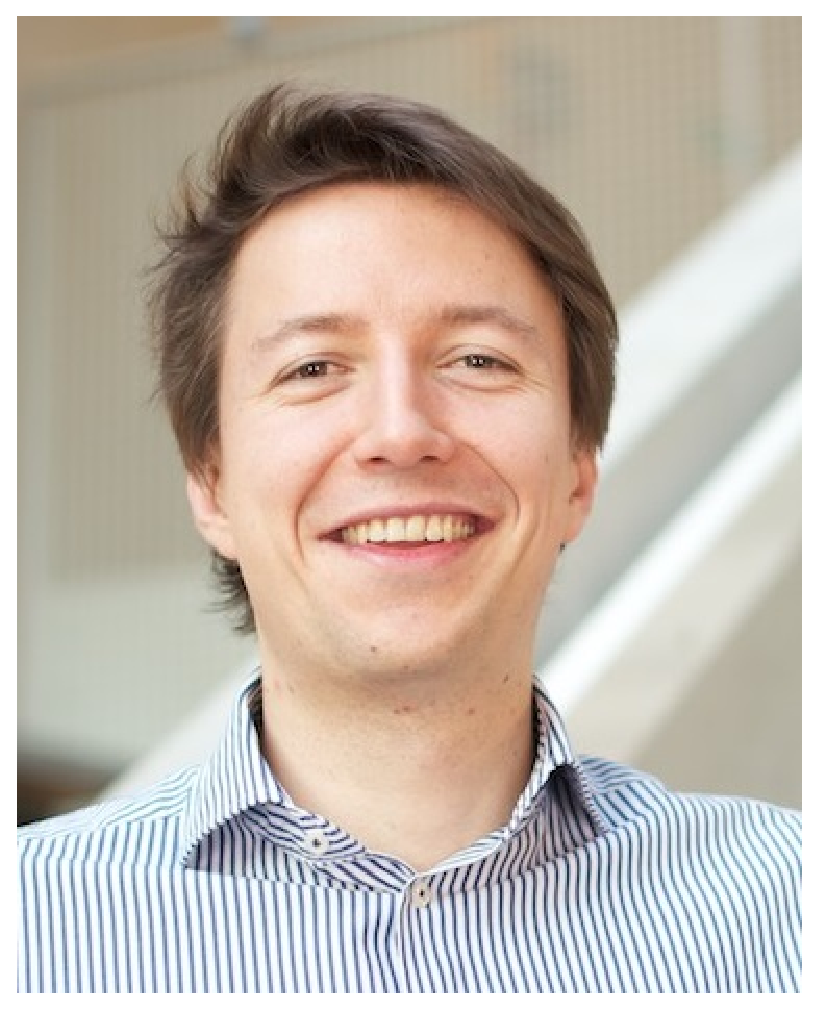
\includegraphics[height=1in]{images/vitae/ckloss}}
\noindent {\bf Christoph Kloss} received his Diploma in Mechatronics in 2007 and his PhD in Computational Fluid Dynamics in 2011, 
both at the Johannes Kepler University in Linz. From 2011 to 2014, he has been Senior Research Associate at the Department of 
Particulate Flow Modelling at the Johannes Kepler University (JKU), where he headed a DEM and CFD-DEM modelling team together 
with Dr. Goniva. Dr. Kloss is co-founder and core developer of the ``CFDEM\textregistered project'', where he is heading the development of the open source DEM code LIGGGHTS\textregistered
Dr. Kloss and Dr. Goniva founded DCS Computing in January 2012. DCS is now a leading company in providing simulation software, 
products and services in the field of DEM and CFD-DEM simulations for a variety of industries. Dr. Kloss is currently holding the position as director of DCS Computing.

\vspace{2cm}

\parpic{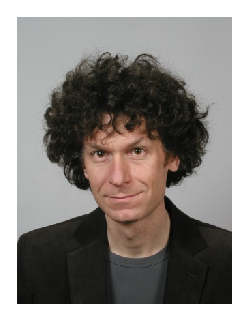
\includegraphics[height=1in]{images/vitae/spirker}}
\noindent {\bf Stefan Pirker} received his PhD in Computational Fluid Dynamics in 2001 at the Johannes Kepler University in Linz/Austria. 
In 2009 he was awarded a Christian-Doppler Laboratory on Particulate Flow Modelling, focusing on numerical modelling of particle laden flows. 
This involves development, experimental validation, application and finally open source distribution of hybrid particle laden flow models. 
After his habilitation in 2011, Stefan Pirker is currently heading the Department of Particulate Flow Modelling at the Johannes Kepler University in Linz/Austria.


\renewcommand\thefigure{\arabic{figure}}

\end{document}
